\chapter{Badania}\label{chap.research}
\section{Wyniki}
Dla operacji \textit{Word Count} wyniki wydajności są przedstawione w tabeli \ref{tab:word-count-results}. Wielkość pliku wsadowego to 4 GB. Można zaobserwować, że operacja na platformie Apache Spark jest około cztery razy szybsza od Apache Hadoop. Wszystkie pomiary poza $time\_starttransfer$ oraz $time\_total$ można uznać za pomijalne dla końcowego użytkownika. Warto też odnotować iż operacja \textit{Word Count} jest najbardziej czasochłonną operacją spośród wszystkich badanych.  
\begin{table}[]
	\centering
	\caption{Wyniki wydajności dla zliczania ilości wystąpień poszczególnych fraz tekstowych (oddzielonych spacją) znalezionych w źródle danych oraz zapisu wyniku do pliku}
	\label{tab:word-count-results}
	\begin{tabular}{|l|l|l|}
		\hline
		Czas [s]    & Hadoop     & Spark      \\ \hline
		time\_namelookup    & 0.000020   & 0.000023   \\ \hline
		time\_connect       & 0.000097   & 0.000116   \\ \hline
		time\_appconnect    & 0.000000   & 0.000000   \\ \hline
		time\_pretransfer   & 0.000116   & 0.000134   \\ \hline
		time\_redirect      & 0.000000   & 0.000000   \\ \hline
		time\_starttransfer & 402.792577 & 111.232410 \\ \hline
		time\_total         & 402.792625 & 111.232446 \\ \hline
	\end{tabular}
\end{table}
\newline Dla operacji \textit{Filter} wyniki wydajności są przedstawione w tabeli \ref{tab:filter-results}. Wielkość pliku wsadowego to 4GB. Operacja \textit{Filter} jest około dwa i pół raza wolniejsza na platformie Apache Hadoop w stosunku do Apache Spark. Również w tym przypadku wszelkie pomiary poza $time\_starttransfer$ oraz $time\_total$ można uznać za pomijalne dla końcowego użytkownika. Operacja \textit{Filter} jest najkrócej trwającą, ze wszystkich badanych. 
\begin{table}[]
	\centering
	\caption{Wyniki wydajności dla zliczania ilości linii zawierających frazę tekstową zdefiniowaną przez użytkownika}
	\label{tab:filter-results}
	\begin{tabular}{|l|l|l|}
		\hline
		Czas [s]    & Hadoop    & Spark     \\ \hline
		time\_namelookup    & 0.000022  & 0.000029  \\ \hline
		time\_connect       & 0.000090  & 0.000113  \\ \hline
		time\_appconnect    & 0.000000  & 0.000000  \\ \hline
		time\_pretransfer   & 0.000110  & 0.000140  \\ \hline
		time\_redirect      & 0.000000  & 0.000000  \\ \hline
		time\_starttransfer & 42.685888 & 16.489812 \\ \hline
		time\_total         & 42.685924 & 16.489860 \\ \hline
	\end{tabular}
\end{table}
\newline Dla operacji \textit{Reject} wyniki wydajności są przedstawione w tabeli \ref{tab:reject-results}. Wielkość pliku wsadowego to 4GB. Operacja \textit{Reject} jest około pięciu razy szybsza dla platformy Apache Spark w stosunku do Apache Hadoop. Tak jak w dwóch poprzednich badanych przypadkach: \textit{Filter} oraz \textit{Word Count} pomiary poza $time\_starttransfer$ oraz $time\_total$ można uznać za pomijalne dla końcowego użytkownika.
\begin{table}[]
	\centering
	\caption{Wyniki wydajności odrzucenia linii zawierających frazę tekstową zdefiniowaną przez użytkownika oraz zapisania wyniku do pliku}
	\label{tab:reject-results}
	\begin{tabular}{|l|l|l|}
		\hline
		Czas [s]    & Hadoop     & Spark     \\ \hline
		time\_namelookup    & 0.000025   & 0.000049  \\ \hline
		time\_connect       & 0.000098   & 0.000184  \\ \hline
		time\_appconnect    & 0.000000   & 0.000000  \\ \hline
		time\_pretransfer   & 0.000118   & 0.000237  \\ \hline
		time\_redirect      & 0.000000   & 0.000000  \\ \hline
		time\_starttransfer & 238.408629 & 45.186254 \\ \hline
		time\_total         & 238.408673 & 45.186296 \\ \hline
	\end{tabular}
\end{table}

\begin{table}[]
	\centering
	\caption{Wyniki wydajności odrzucenia linii zawierających frazę tekstową zdefiniowaną przez użytkownika oraz zapisania wyniku do pliku na platformie Apache Spark ze względu na zastosowanie strategi przechowywania RDD.}
	\label{tab:reject-spark-modes-results}
	\begin{tabular}{|l|l|l|}
		\hline
		Czas{[}s{]}         & Dysk twardy & Pamięć RAM \\ \hline
		time\_namelookup    & 0.000029    & 0.000049   \\ \hline
		time\_connect       & 0.000106    & 0.000184   \\ \hline
		time\_appconnect    & 0.000000    & 0.000000   \\ \hline
		time\_pretransfer   & 0.000140    & 0.000237   \\ \hline
		time\_redirect      & 0.000000    & 0.000000   \\ \hline
		time\_starttransfer & 162.751406  & 45.186254  \\ \hline
		time\_total         & 162.751459  & 45.186296  \\ \hline
	\end{tabular}
\end{table}

\begin{table}[]
	\centering
	\caption{Wyniki wydajności dla zliczania ilości linii zawierających frazę tekstową zdefiniowaną przez użytkownika na platformie Apache Spark ze względu na zastosowanie strategi przechowywania RDD.}
	\label{tab:word-occurence-spark-modes-results}
	\begin{tabular}{|l|l|l|}
		\hline
		Czas{[}s{]}         & Dysk twardy & Pamięć RAM \\ \hline
		time\_namelookup    & 0.000021    & 0.000029   \\ \hline
		time\_connect       & 0.000096    & 0.000113   \\ \hline
		time\_appconnect    & 0.000000    & 0.000000   \\ \hline
		time\_pretransfer   & 0.000115    & 0.000140   \\ \hline
		time\_redirect      & 0.000000    & 0.000000   \\ \hline
		time\_starttransfer & 51.502827   & 16.489812 \\ \hline
		time\_total         & 51.502860   & 16.489860 \\ \hline
	\end{tabular}
\end{table}

\begin{table}[]
	\centering
	\caption{Wyniki wydajności dla zliczania ilości wystąpień poszczególnych fraz tekstowych (oddzielonych spacją) znalezionych w źródle danych oraz zapisu wyniku do pliku na platformie Apache Spark ze względu na zastosowanie strategi przechowywania RDD.}
	\label{tab:word-count-spark-modes-results}
	\begin{tabular}{|l|l|l|}
		\hline
		Czas{[}s{]}         & Dysk twardy & Pamięć RAM \\ \hline
		time\_namelookup    & 0.000023    & 0.000023   \\ \hline
		time\_connect       & 0.000099    & 0.000116   \\ \hline
		time\_appconnect    & 0.000000    & 0.000000   \\ \hline
		time\_pretransfer   & 0.000118    & 0.000134   \\ \hline
		time\_redirect      & 0.000000    & 0.000000   \\ \hline
		time\_starttransfer & 144.407036  & 111.232410 \\ \hline
		time\_total         & 144.407089  & 111.232446 \\ \hline
	\end{tabular}
\end{table}
Tabele \ref{tab:word-count-results}, \ref{tab:filter-results}, \ref{tab:reject-results} przedstawiają porównanie wszystkich badanych operacji na platformach Apache Hadoop oraz Apache Spark skonfigurowanych w sposób, który jest skalibrowany na najwyższą wydajność. W sekcji \ref{RDD-strategy} przedstawione są możliwe warianty konfiguracji platformy Apache Spark. Podczas badań zostały dokonane pomiary również w trybie wykorzystania dysku twardego do przechowywania zbioru danych RDD. Różnice w wydajności ze względu na zastosowaną strategie dla każdej badanej operacji można zaobserwować w tabelach \ref{tab:reject-spark-modes-results}, \ref{tab:word-occurence-spark-modes-results}, \ref{tab:word-count-spark-modes-results}. Wyniki zostały uzyskane na podstawie tego samego pliku wsadowego, który był wykorzystany do uzyskania wyników z tabel  \ref{tab:word-count-results}, \ref{tab:filter-results}, \ref{tab:reject-results}. Można zaobserwować, że wykorzystanie innej strategii przechowywania zbioru RDD znacząco wpływa na wydajność operacji na platformie Apache Spark. Dla operacji \textit{Reject} korzystanie ze strategii zapisu danych na dysku twardym owocuje o około 3,5 raza wolniejszym wykonywaniem. Dla operacji \textit{Filter}  zastosowanie tej samej strategii jest wolniejsze o około 3,1 raza niż strategii pamięci RAM. Operacja \textit{Word Count} traci na wydajności najmniej spośród wszystkich badanych - około 1,3 raza.  
\section{Interpretacja wyników}
Z punktu widzenia badanej wydajności wszystkie pomiary poza \textbf{time\_starttransfer} oraz \textbf{time\_total} nie są kluczowe gdyż pomijają czas pracy badanych platform. Czas całkowity jest interesujący z punktu widzenia użytkownika systemu, którego interesuje faktyczny czas uzyskania wyników. Podczas interpretacji wyników mylący może być opis przedstawiony w \ref{items:time-descriptions} \textit{Czas przed którym pierwszy bajt danych miał zostać wysłany}. Opis ten nie dotyczy danych, które są przetwarzane na badanych platformach lecz danych wysłanych przez odpowiedź na żądanie HTTP. Oznacza to, że dane odpowiedzi zostały wysłane po czasie gdy wszystkie obliczenia na platformie zostały już wykonane. W związku z tym \textbf{time\_starttransfer} może zostać uznany za czas pracy przetwarzania na danej platformie.
\newline W związku z wynikami przedstawionymi w tabelach \ref{tab:filter-results}, \ref{tab:reject-results}, \ref{tab:word-count-results} możemy zaobserwować zależność, że platforma Spark jest zdecydowanie szybsza (od dwóch i pół do pięciu razy) jeżeli chodzi o wykonywanie obliczeń i zapis wyników do pliku w systemie HDFS. Porównanie wydajności wszystkich operacji dla najbardziej wydajnej strategii przechowywania danych jest przedstawione na rysunku \ref{fig:results-comparison-bar}.
\begin{figure}[!htb]
	\centering
	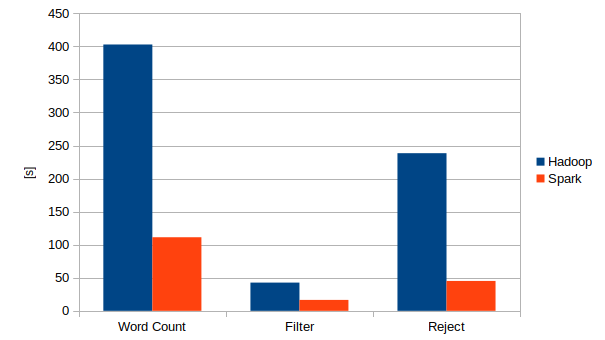
\includegraphics[scale=0.6]{results-comparison-bar.png}
	\caption{Wyniki wydajności operacji: Word Count, Filter i Reject na platformach Apache Spark oraz Apache Hadoop dla najbardziej wydajnej strategii przechowywania danych.}
	\label{fig:results-comparison-bar}
\end{figure}
Zauważalna wyższa wydajność platformy Apache Spark wynika z zastosowania strategii przechowania danych w pamięci RAM. Dzięki dokonywaniu obliczeń w pamięci RAM unikana jest mnogość operacji wejścia oraz wyjścia co skutkuje zauważalną różnicą w wydajności.
\begin{figure}[!htb]
	\centering
	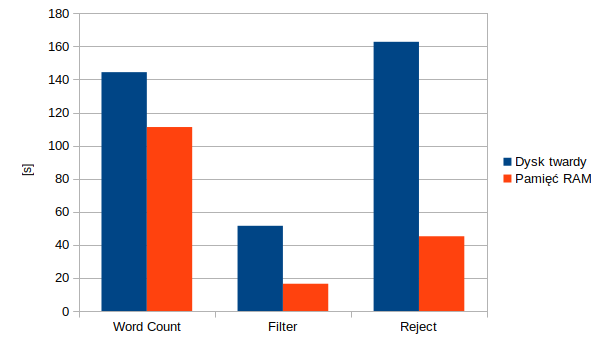
\includegraphics[scale=0.6]{results-spark-strategy-comparison-bar.png}
	\caption{Wyniki wydajności operacji: Word Count, Filter i Reject na platformie Apache Spark ze względu na zastosowaną strategię przechowywania danych.}
	\label{fig:results-spark-strategy-comparison-bar}
\end{figure}
Na rysunku \ref{fig:results-spark-strategy-comparison-bar} zostały przedstawione wyniki wszystkich operacji ze względu na zastosowaną strategię przechowywania danych w pamięci RAM lub na dysku twardym. Można zaobserwować, że wydajność operacji jest zróżnicowana w zależności od jej rodzaju. Na podstawie wykonanych badań można jednoznacznie stwierdzić, że operacje na dysku twardym będą zawsze wolniejsze od tych wykonywanych w pamięci RAM. Jednocześnie nie można ustalić jednoznacznej wartości, która pozwala wyznaczyć spadek wydajności podczas zastosowania strategii dysku twardego. Na podstawie wykonanych badań można stwierdzić, że zastosowanie strategii dysku twardego powoduje spadek wydajności od 1,3 do 3,5 raza i jest zależne od rodzaju operacji. 
\begin{figure}[!htb]
	\centering
	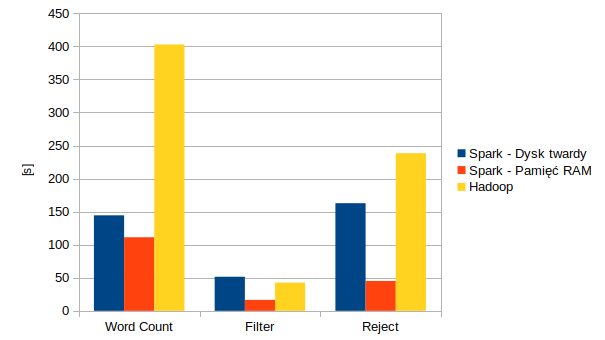
\includegraphics[scale=0.6]{results-comparison-bar-all.png}
	\caption{Wyniki zbiorcze wszystkich operacji wykonanych podczas badań.}
	\label{fig:results-comparison-bar-all}
\end{figure}
Na podstawie rysunku \ref{fig:results-comparison-bar-all} można jednoznacznie stwierdzić, że platforma Apache Hadoop jest najmniej wydajną spośród badanych w tej pracy magisterskiej. Niezależnie od zastosowanej operacji czas wykonywania był za każdym razem najdłuższy dla Apache Hadoop. Najbardziej wydajną platformą jest Apache Spark, który stosuje strategię przechowywania danych w pamięci RAM.    
\section{Koszty rozwoju oprogramowania i zasobów ludzkich}\label{development_human_resources}
Badane platformy Apache Spark oraz Apache Hadoop są przedstawicielami dwóch języków programowania dedykowanych na platformę JVM: Scala oraz Java. Apache Spark jest narzędziem napisanym w języku Scala i posiada interfejs programistyczny dla czterech języków programowania: Scala, Java, Python oraz R. Apache Hadoop to narzędzie oparte wyłącznie na języku Java. Rozwijanie systemów informatycznych wiąże się z wieloma aspektami takimi jak: koszty rekrutacji inżynierów posiadających wiedzę z wąskiej dziedziny np. język programowania, ramy projektowej, poszczególnych bibliotek. Innym aspektem długofalowego projektu informatycznego jest pozostawienie możliwości na rozszerzanie rozwiązania oraz integracja z innymi platformami bądź językami programowania. W przypadku Apache Hadoop rozwiązanie jest zamknięte na język Java i integracja z innymi językami programowania wymaga serializacji danych bądź też ich zapisu we wcześniej uzgodnionym formacie na przykład HDFS. W przypadku Apache Spark prace implementacji systemu mogą być prowadzone w kilku językach. Dodatkowo można wykorzystywać zaletę samego języka Scala, gdzie wszystkie biblioteki z języka Java są dostępne i nie wymagają żadnego dodatkowego nakładu pracy przy ich użyciu. W kontekście tej pracy magisterskiej zostały wykonane implementacje tych samych funkcjonalności dla dwóch języków Scala i Java. Operacja zliczenia wystąpień danej frazy w linii dla języka Scala została przedstawiona w listingu \ref{lst:scala-occurence-listing}. Ta sama operacja dla języka Java została przedstawiona w listingu \ref{lst:java-occurrence-listing}.
\begin{lstlisting}[language=scala, caption={Operacja zliczania wystąpień danej frazy w linii dla języka Scala na platformie Apache Spark},captionpos=b, label={lst:scala-occurence-listing}]
class WordOccurrence {
	def run(sparkContext: SparkContext, filePath: String, word: String) = {
	val lines: RDD[String] = sparkContext.textFile(filePath)
	val linesContainingWord = lines.filter(line => line.contains(word))
	linesContainingWord.count()
	}
}
\end{lstlisting}
\begin{lstlisting}[language=Java, caption={Operacja zliczania wystąpień danej frazy w linii dla języka Java na platformie Apache Hadoop},captionpos=b, label={lst:java-occurrence-listing}]
public class WordOccurrence {

public long run(String basePathHDFS, String wordToBeFound) throws Exception {
Path pt = new Path(basePathHDFS + "mergedTweets0.3686418061949279.txt");
Configuration conf = new Configuration();
conf.set("fs.defaultFS", basePathHDFS);
conf.set("wordToBeFound", wordToBeFound);
Job job = new Job(conf, "WordOccurrence");
job.setOutputKeyClass(Text.class);
job.setOutputValueClass(IntWritable.class);

job.setMapperClass(FilterMapper.class);
job.setReducerClass(SimpleReduce.class);

job.setInputFormatClass(TextInputFormat.class);
job.setOutputFormatClass(TextOutputFormat.class);

FileInputFormat.addInputPath(job, pt);
TimeStamp myTs = TimeStamp.getCurrentTime();
FileOutputFormat.setOutputPath(job, new Path(basePathHDFS + "hadoopWordOccurrenceResult" + myTs));
job.waitForCompletion(true);
return job.getCounters().findCounter("org.apache.hadoop.mapred.Task$Counter", "MAP_OUTPUT_RECORDS").getValue();
}

}

public class FilterMapper extends Mapper<LongWritable, Text, Text, IntWritable> {
private final IntWritable one = new IntWritable(1);
private Text word = new Text();

public void map(LongWritable key, Text value, Context context) throws IOException, InterruptedException {
String wordToBeFound = context.getConfiguration().get("wordToBeFound");
String line = value.toString();
if (line.contains(wordToBeFound)) {
context.write(word, one);
}
}
}
public class SimpleReduce extends Reducer<Text, IntWritable, Text, IntWritable> {
public void reduce(Text key, Iterable<IntWritable> values, Context context)
throws IOException, InterruptedException {
int sum = 0;
for (IntWritable val : values) {
sum += val.get();
}
context.write(key, new IntWritable(sum));
}
}
\end{lstlisting}
Nie trudno zauważyć, że ta sama funkcjonalność dla języka Scala może być przedstawiona o wiele bardziej zwięźle i czytelnie niż w języku Java. Sama różnica w ilości kodu jest zauważalna - Scala 7 linii, Java 48 linii. W przypadku utrzymywania kodu jest to bardzo ważne by rozwiązania były czytelne i łatwe do opanowania. Szczególnie istotne jest to w dużych projektach, gdzie inżynierowie często zmieniają odpowiedzialność za dany fragment funkcjonalności, bądź też występuje duża rotacja programistów. Wybór języka programowania, może też mieć znaczący wpływ na koszty rozwoju oraz utrzymania danego projektu informatycznego z racji na różnice w zarobkach ze względu na technologię. Na wykresach \ref{fig:@=salaries_contract} oraz \ref{fig:@=salaries_permanent} możemy zobaczyć koszty zatrudniania inżynierów ze względu na technologię oraz rodzaj zatrudnienia w latach 2015, 2016 oraz 2017 na terenie Wielkiej Brytanii. Dane zostały pobrane z serwisu internetowego \url{https://www.itjobswatch.co.uk}.
\begin{figure}[h]
	\centering
	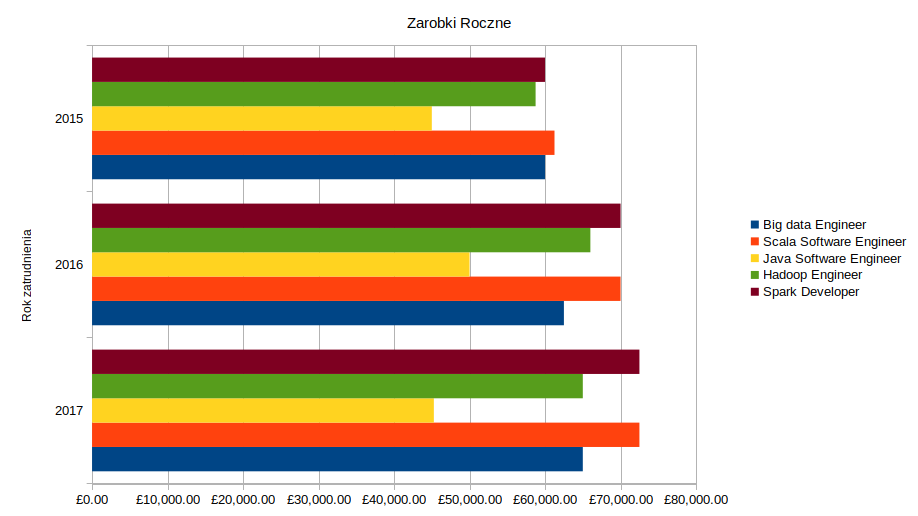
\includegraphics[scale=0.5]{salaries_contract.png}
	\caption{Trendy zarobków rocznych na terenie Wielkiej Brytanii w latach 2015, 2016 oraz 2017 dla formy zatrudnienia na kontrakt.}
	\label{fig:@=salaries_contract}
\end{figure}
\begin{figure}[h]
	\centering
	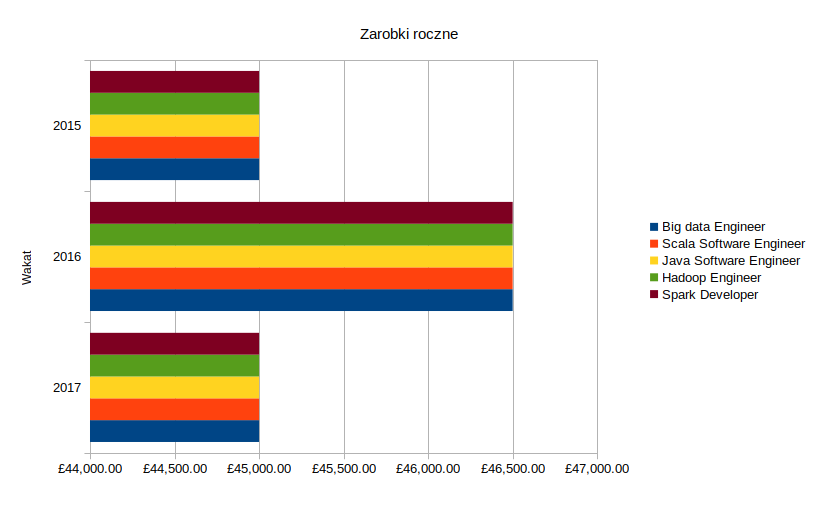
\includegraphics[scale=0.5]{salaries_permanent.png}
	\caption{Trendy zarobków rocznych na terenie Wielkiej Brytanii w latach 2015, 2016 oraz 2017 dla formy zatrudnienia stałego (umowy o pracę).}
	\label{fig:@=salaries_permanent}
\end{figure}
\newline Na podstawie rysunku \ref{fig:@=salaries_permanent} możemy zauważyć, że w kontekście rekrutacji ze względu na narzędzie bądź język programowania nie występują różnice płac dla stałej formy zatrudnienia. Jest to szczególnie istotne dla projektów o charakterystyce długofalowej oraz dużej wielkości. W przypadku formy zatrudniania stałego pracowników i dużych projektach można wybrać dowolną technologię, gdyż koszty będą relatywnie takie same (wyniki to średnie płac na dane stanowisko). Przedsiębiorstwo może również wybrać tą technologię bądź język programowania, który jest opanowany przez największą grupę docelową na rynku pracy tak by zwiększyć swoje możliwości rekrutacyjne.\newline Zupełnie odwrotnie przedstawia się sytuacja dla okresowej formy zatrudnienia tak zwany kontrakt. Dokładne dane dotyczące formy zatrudnienia na kontrakt są widoczne na rysunku \ref{fig:@=salaries_contract}. Można zaobserwować zróżnicowane płac rocznych ze względu na narzędzie bądź język programowania sięga dwudziestu siedmiu i pół tysiąca funtów rocznie. W ostatnich trzech latach najtańsze były osoby zatrudnione na kontrakt znające język programowania Java. Drugie miejsce od końca najwyższych płac rocznych zajmują inżynierowie znający Apache Hadoop. Najdroższe osoby to te posiadające kompetencje w platformie Apache Spark. 